\documentclass[a4paper,12pt,french]{book}
\usepackage[margin=2cm]{geometry}
\usepackage[thinfonts]{uglix2}

\usepackage{array}
\newcommand{\tabstrut}{\vrule height 1.25em depth 0.5em width 0pt}
\begin{document}
\setcounter{chapter}{3}
\chapter{\large Arithmétique\\[-1em]\fontsize{35pt}{42pt}\selectfont\titlefont Arithmétique modulaire}

\section{Entiers naturels et division euclidienne}

\begin{definition}[ (rappel) : ensemble des entiers naturels]
	On note $\N$ l'ensemble des \textit{entiers naturels}. $$\N=\lbrace 0;1;2;3;4;5;6;7;8;9;10;11;12\ldots\}$$
\end{definition}

\begin{definition}[ (rappel) : division euclidienne dans \N]
	
	Soient A et B deux entiers naturels, et $B\neq 0$. Il existe deux nombres uniques Q et R (vérifiant $0\geqslant R<B$) tels que l'on puisse écrire
	$$A = Q\times B + R$$
	
	C'est exactement la division que l'on a apprise en sixième (celle où l'on s'arrête aux nombres entiers):
	\begin{center}
		\begin{tabular}{r|l}
			A & B\\
			\cline{2-2}
			R & Q
		\end{tabular}
		
		\begin{enumerate}[\textbullet]
			\item 	A est appelé le \textit{dividende};
			\item 	B est le \textit{diviseur};
			\item	Q est le \textit{quotient};
			\item 	R est le \textit{reste}, il est \textit{impérativement} plus petit que B.
		\end{enumerate}
	\end{center}
\end{definition}

\begin{exemple}[s]
	Effectuons la division euclidienne de 27 par 7 :
		\begin{center}
		\begin{tabular}{r|l}
			27 & 7\\
			\cline{2-2}
			6 & 3
		\end{tabular}
		\end{center}
	Ainsi on a $\displaystyle\underbrace{27}_{A}=\underbrace{3}_{Q}\times \underbrace{7}_{B}+\underbrace{6}_{R}$.\\[3em]
	
	Effectuons la division euclidienne de 297 par 11 :
	\begin{center}
		\begin{tabular}{r|l}
			297 & 11\\
			\cline{2-2}
			0 & 27
		\end{tabular}
	\end{center}
	Ainsi on a $\displaystyle\underbrace{286}_{A}=\underbrace{26}_{Q}\times \underbrace{11}_{B}+\underbrace{0}_{R}$.
\end{exemple}

\begin{exercice}[]
	Effectuer les divisions euclidiennes suivantes :
	\begin{multicols}{4}
		\begin{enumerate}[\bfseries a.]
			\item 	28 par 8
			\item 	100 par 9
			\item 	379 par 11
			\item 	427 par 13\\
		\end{enumerate}
	\end{multicols}
\end{exercice}



\begin{definition}[ : diviseurs et multiples]
	Quand la division euclidienne de A par B donne un reste nul (lorsqu'elle tombe juste) on dit que \emph{B est un diviseur de A} ou bien (ce qui revient au même) que \emph{A est un multiple de B}.
\end{definition}

\begin{exemple}[s]
	\begin{enumerate}[\textbullet]
		\item 	$27 = 3\times 7 +4$ donc 7 ne divise pas 27 (7 n'est pas \textit{un diviseur} de 27).\\
				On peut dire aussi que 27 n'est pas multiple de 7.
		\item 	$286 = 26\times 11+0$ donc 1 est donc un diviseur de 286.
	\end{enumerate}
\end{exemple}
\begin{remarque}[s]
	\begin{enumerate}[\bfseries a.]
		\item 	$28 = 4\times 5 +8$ mais ce n'est pas la division euclidienne de 28 par 5 car le \og reste\fg{} 8 n'est pas plus petit que 5.
				\begin{tabbing}
					$28$ 	\= 	$=4\times 5 + 8$\\
							\>	$=4\times 5 + 5 + 3$\\
							\>	$=5\times 5 +3\qquad$ voilà la division euclidienne.
				\end{tabbing}
		\item 	\textit{\og une division euclidienne n'en donne pas toujours 2\fg{}	} :\\
				$27 = 3\times 7 + 4$ est la division euclidienne de 27 par 7.\\
				On peut réarranger : $27 = 7\times 3 +4$ mais ce n'est pas la division euclidienne de 27 par 3  car le reste est trop grand.\\
				
				Ceci dit quand le reste est suffisamment petit, on obtient \og 2 divisions pour le prix d'une \fg{}:
				$162=12\times 13 +1$ est la division euclidienne de 162 par 12, et de 162 par 13 aussi.
				
		\item 	\textit{\og une division euclidienne qui tombe juste en donne deux en général\fg{}} :\\
				$297=27\times 11$ nous donne 2 diviseurs de 297 : 27 et 11.\\
				$16 = 4\times4$ aussi... mais c'est deux fois le même !
		\item 	avec la calculatrice, pour savoir si $B$ divise $A$ il suffit d'entrer $A\div B$ et de regarder si le résultat est entier.
	\end{enumerate}
\end{remarque}



\begin{exercice}[]
	Les égalités suivantes, peuvent-elles être des divisions euclidiennes ?\\
	Si oui, préciser A, B, Q et R.
	\begin{multicols}{4}
		\begin{enumerate}[\bfseries a.]
			\item 	$65=32\times 2 +1$
			\item 	$80=5\times 10 + 30$
			\item 	$100 = 9\times 11 +1$
			\item 	$17=    3\times4 +5	$\\
		\end{enumerate}
	\end{multicols}
\end{exercice}

\begin{exercice}[]
	
	Les égalités suivantes ne sont pas des divisions euclidiennes.\\
	Transformez-les pour qu'elles le deviennent (il peut y avoir plusieurs possibilités).
	
	\begin{multicols}{4}
		\begin{enumerate}[\bfseries a.]
			\item 	$19=3\times 4 + 7$
			\item 	$30=2\times 10 + 10$
			\item 	$29 = 4\times 5 +9$
			\item 	$23=  4\times 7 -5$\\
		\end{enumerate}
	\end{multicols}
\end{exercice}



\begin{pythoncode}
>>> a = 17   # déclare une variable a de type int (entier)
>>> b = 5    # idem avec b
>>> q = a // b # // donne le quotient par b
>>> r = a % b  # %  donne le reste modulo b
>>> print(q)
5
>>> print(r)
2
\end{pythoncode}
\section{Diviseurs et nombres premiers}

\begin{propriete}
Soient $a$ et $b$ deux entiers naturels. Dire que $b$ est un diviseur de $a$ veut dire que la division euclidienne de $a$ par $b$ donne un reste nul.\\
Cela signifie donc qu'il existe un entier naturel $k$ tel que $$a=k\times b$$
On peut également dire que $a$ est multiple de $b$
\end{propriete}

\begin{remarque}
	Si $b$ divise $a$ il existe un entier naturel $k$ tel que $$a=k\times b$$ et donc $k$ divise $a$ également.
\end{remarque}

\begin{exemple}[]
	$20=5\times 4$ donc 5 et 4 sont deux diviseurs de 20.
\end{exemple}

\begin{exercice}[]
	
	À l'aide de la calculatrice (ou non), déterminer si $b$ divise $a$.
	\begin{enumerate}[\bfseries a.]
		\item 	$a=251$ et $b=13$
		\item 	$a=8$ et $b=80$
		\item 	$a=111$ et $b=37$
		\item 	$a=131072$ et $b=8192$\\
	\end{enumerate}
	
\end{exercice}


\begin{propriete}[s]
	\begin{enumerate}[\bfseries a.]
		\item 	Si a est divisible par b alors tout multiple de a est également divisible par b.
		\item 	Si a est divisible par b et que b est divisible par c alors a est divisible par c.
		\item 	Si a et b sont divisibles par c alors a+b aussi et (si a>b)  a-b aussi.
	\end{enumerate}
\end{propriete}
\begin{exemple}[s]
	\begin{enumerate}[\bfseries a.]
		\item 	12 est divisible par 3 donc tout multiple de 12 aussi : \np{12000} est donc divisible par 3.
		\item 	120 est divisible par 12 et 12 est divisible par 3 donc 120 est divisible par 3.
		\item 	Puisque \np{12000} et 12 sont divisibles par 3, \np{12000}-12, soit \np{11988}, l'est aussi.
	\end{enumerate}
\end{exemple}
\begin{definition}[ : entier naturel premier]
	Un entier naturel est dit \textit{premier} lorsqu'il admet 2 diviseurs \textit{distincts} : 1 et lui-même.
	\begin{enumerate}[\textbullet]
		\item 	0 n'est pas premier : $0=1\times 0=2\times 0=3\times 0=...$
		\item 	1 n'a qu'un diviseur : lui-même. Il n'est pas premier.
		\item 	2 est premier.
		\item 	3 aussi.
		\item 	4 ne l'est pas car 1, 2 et 4 divisent 1.
	\end{enumerate}
\end{definition}

Il est assez simple de montrer qu'il y a une infinité de nombres premiers. Les nombres premiers jouent un rôle très important en mathématiques et interviennent dans les systèmes de cryptographie (basiques ou sophistiqués).

\begin{exercice}[ : crible d'\'Eratosthène]
	
	Dans la grille suivante :
	\begin{enumerate}[\textbullet]
		\item 	Entourer 2 et barrer 2 et tous ses multiples.
		\item 	Une fois cela fait, 3 est le premier nombre non barré après 2 donc on l'entoure et on barre tous ses multiples.
		\item 	Continuer jusqu'à ce que tous les nombres de la grilles soient traités (soit barrés soit entourés).
		\item 	Les nombres entourés sont \textit{des nombres premiers}.
	\end{enumerate}
	\begin{center}
		\xdef\x{0}
		\begin{tabular}{|*{10}{>{\tabstrut\xdef\x{\the\numexpr\x+1\relax}\ifnum\x=1 \else\x\fi}c|}}
			\hline
			&&&&&&&&&\\
			\hline
			&&&&&&&&&\\
			\hline
			&&&&&&&&&\\
			\hline
			&&&&&&&&&\\
			\hline
			&&&&&&&&&\\
			\hline
			&&&&&&&&&\\
			\hline
			&&&&&&&&&\\
			\hline
			&&&&&&&&&\\
			\hline
			&&&&&&&&&\\
			\hline
			&&&&&&&&&\\
			\hline
		\end{tabular}
	\end{center}
	
	Recopier ici la liste des nombres premiers trouvés :\\[4em]
	
	
\end{exercice}



\begin{propriete}[]
	Soit $n$ un entier supérieur ou égal à 2 :\begin{enumerate}[\textbullet]
		\item 	ou bien $n$ possède un diviseur inférieur ou égal à $\sqrt{n}$ et, à ce moment là, $n$ \textit{n'est pas premier.}
		\item 	ou bien \textit{aucun nombre premier } inférieur à $\sqrt{n}$ ne divise $n$ et \textit{il est premier}.
	\end{enumerate}
\end{propriete}



\begin{methode}[ : déterminer si un nombre est premier ou non]
	Voici le début de la liste des nombres premiers :
	$$\lbrace 2;\ 3;\ 5;\ 7;\ 11;\ 13;\ 17;\ 19\rbrace$$
	\begin{enumerate}[\textbullet]
		\item 	133 est-il premier ?\\
		
				$\sqrt{133}\approx 11,5$ donc on regarde si 133 est divisible par 2, 3, 5, 7 ou 11.\\
				On trouve que 133 = $19\times 7$ donc 133 n'est pas premier.
		\item 	251 est-il- premier ?\\
				$\sqrt{251}\approx 15,8$ donc on regarde si 251 est divisible par 2, 3, 5, 7, 11, ou 13.\\
				Ce n'est pas le cas : 251 est donc premier.
	\end{enumerate}
\end{methode}

\begin{exercice}[]
	
	
	Les nombres suivants sont ils premiers ?
	
	\begin{multicols}{3}
		\begin{enumerate}[\bfseries a.]
			\item 143
			\item 145
			\item 141
			\item 147
			\item 247
			\item 257
		\end{enumerate}
	\end{multicols}
	
\end{exercice}


\begin{propriete}[ : décomposition en produit de facteurs premiers]
	Tout entier naturel supérieur ou égal à 2 se décompose de manière unique (à l'ordre près) en \textit{produit de facteurs premiers}.
\end{propriete}

\begin{methode}[]
	Pour décomposer un nombre en produit de facteurs premiers, on cherche n'abord ses petits diviseurs premiers et on recommence jusqu'à trouver 1 :
	\begin{center}
		\begin{tabular}{r|l}
			234 & 2 \hspace*{3ex}on voit que 234 est pair\\
			117 & 3 \hspace*{3ex}car 3 est le plus petit nombre premier qui divise 117\\
			39 & 3 \hspace*{3ex}et ainsi de suite \\
			13 & 13\hspace*{3ex}...\\
			1 & \hspace*{4.55ex}on arrête
		\end{tabular}
	\end{center}
	On a donc 	
	\begin{tabbing}
		234 \= $=2\times 3\times 3\times 13$\\ 
		\> $=2\times 3^2\times 13\qquad$ et c'est la décomposition en produit de facteurs premiers de 234.
	\end{tabbing}
\end{methode}



\begin{exercice}[]
	
	Décomposer les nombres suivants en produit de facteurs premiers.
	
	\begin{multicols}{4}
		\begin{enumerate}[\bfseries a.]
			\item 30
			\item 60
			\item 96
			\item 684
		\end{enumerate}
	\end{multicols}
	
\end{exercice}


\begin{methode}[ : liste des diviseurs d'un entier]
	Pour trouver \textit{tous} les divieurs d'un entier supérieur ou égal à 2 :
	\begin{enumerate}[\bfseries a.]
		\item 	on le décompose en produit de facteurs premiers.
		\item 	on écrit tous les nombres que l'on peut former en prenant \og moins de facteurs\fg{} dans cette décomposition.
	\end{enumerate}
\end{methode}

\begin{exemple}[]
	Trouvons tous les diviseurs de 60 : \\
	$60=2\times30=2^2\times 15=2^2\times 3\times 5$.
	Ses diviseurs sont donc \\
	
	\begin{tabular}{l|l}
		1 & $2^0\times 3^0\times 5^0$\\
		5 & $2^0\times 3^0\times 5^1$\\
		3 & $2^0\times 3^1\times 5^0$\\
		15 & $2^0\times 3^1\times 5^1$\\
		2 & $2^1\times 3^0\times 5^0$\\
		10 & $2^1\times 3^0\times 5^1$\\
		6 & $2^1\times 3^1\times 5^0$\\
		30 & $2^1\times 3^1\times 5^1$\\
		4 & $2^2\times 3^0\times 5^0$\\
		20 & $2^2\times 3^0\times 5^1$\\
		12 & $2^2\times 3^1\times 5^0$\\
		60 & $2^2\times 3^1\times 5^1$\\
		\end{tabular}
\end{exemple}

Il est très facile d'oublier des diviseurs. Pour que cela n'arrive pas il faut utiliser une méthode logique pour les énumérer.\\
Voici un exemple d'algorithme qui les donne tous, en reprenant l'exemple de 60.\newpage

\begin{verbatim}
Variables
i, j, k : entiers
Début
    Pour i allant de 0 à 2
        Pour j allant de 0 à 1
            Pour k allant de 0 à 1
                Afficher 2^i * 3^j * 5^k
            FinPour
        FinPour
    FinPour
Fin
\end{verbatim}


\begin{exercice}[]
	
	Donner la liste des diviseurs des nombres suivants.
	
	\begin{multicols}{4}
		\begin{enumerate}[\bfseries a.]
			\item 30
			\item 25
			\item 96
			\item 684
		\end{enumerate}
	\end{multicols}
	
\end{exercice}


\section{pgcd de deux entiers naturels non nuls}

Deux entiers naturels non nuls ont au moins un diviseur commun : 1. Parmi tous les nombres qui les divisent tous les deux il y en a un plus grand : leur pgcd.

\begin{definition}[]
	Soient $a$ et $b$ deux entiers naturels non nuls.\\
	On note $pgcd(a;b)$ et on lit \og pgcd de $a$ et de $b$\fg{} le plus grand entier qui divise à la fois $a$ et $b$.
\end{definition}

\begin{exemple}[s]
	Le plus grand nombre qui divise à la fois 12 et 16, c'est 4. Ainsi $pgcd(12;16)=4$.\\
	25 et 27 n'ont aucun diviseur commun plus grand que 1 : $pgcd(25;27)=1$.\\
\end{exemple}

\begin{definition}[]
	Lorsque $pgcd(a;b)=1$ on dit que $a$ et $b$ sont \textit{premiers entre eux}.
\end{definition}

\begin{exemple}[s]
	25 et 27 sont premiers entre eux. 8 et 15 aussi.
\end{exemple}

\begin{remarque}[]
	Il ne faut pas confondre \textit{nombre premier} (tout court) et \textit{nombres premiers entre eux} :
	\begin{enumerate}[\textbullet]
		\item 	25 et 27 sont premiers entre eux mais aucun de ces deux nombres n'est premier.
		\item 	3 et 30 ne sont pas premiers entre eux : leur pgcd vaut 3. Pourtant 3 est premier.
	\end{enumerate}
\end{remarque}

\begin{methode}[]
	Soient $a$ et $b$ deux entiers naturels que l'on a décomposés en produit de facteur premiers :
	\begin{enumerate}[\textbullet]
		\item 	S'ils n'ont aucun facteur commun alors ils sont premiers entres eux.
		\item 	Sinon, on fait le produit des facteurs communs avec la plus petite puissance qui apparaît dans chacune des décompositions.
	\end{enumerate}
\end{methode}

\begin{exemple}[]
	On veut $pgcd(240;72)$.
	\begin{enumerate}[\textbullet]
		\item 	On commence par décomposer 240 : $240=2^4\times 3^1\times 5^1$.
		\item 	On fait de même pour 72 : $72 = 2^3\times3^2$
		\item 	Il y a deux facteurs premiers en commun dans cette décomposition : 2 et 3. On garde à chaque fois l'exposant le plus petit et on en fait le produit : $$pgcd(a;b)=2^3\times 3^1=24$$	\end{enumerate}
\end{exemple}


\begin{exercice}
	
	En utilisant les décompositions en produit de facteurs premiers, donner le \textsc{PGCD} de 
	
	\begin{multicols}{4}
		\begin{enumerate}[\bfseries a.]
			\item 15 et 27
			\item 63 et 99
			\item 222 et 148
			\item 192 et 69
		\end{enumerate}
	\end{multicols}
	
\end{exercice}


\begin{propriete}[]
	Soient $a$ et $b$ 2 entiers non nuls. Si $b<a$ et qu'on effectue la division euclidienne de $a$ par $b$, on obtient $$a = q\times b +r$$ et à ce moment là
	$$pgcd(a;b)=pgcd(b;r)$$
\end{propriete}
\begin{methode}[ : Algorithme d'Euclide]
	Cette méthode se base sur la propriété précédente. On veut trouver le pgcd de 420 et 182.
	\begin{tabbing}
		$420$ 	\= $=2\times 182+56\qquad$ \= donc $pgcd(420;182)=pgcd(182,56)$ et on recommence.\\
		$182$	\>= $=3\times 56+14$ \>  donc $pgcd(182,56)=pgcd(56,14)$ et on poursuit.\\
		$56$	\> $=3\times 14+\boxed{0}$ \> et on s'arrête.
	\end{tabbing}
	La dernière ligne nous indique que $pgcd(56;14)=14$, ainsi $pgcd(420;182)=14$.
\end{methode}


\begin{exercice}[]
	
	En utilisant la méthode de votre choix, donner le \textsc{PGCD} de 
	
	\begin{multicols}{4}
		\begin{enumerate}[\bfseries a.]
			\item 198 et 256
			\item 546 et 230
			\item 180 et 105
			\item 357 et 399
		\end{enumerate}
	\end{multicols}
	
\end{exercice}



\begin{exercice}[]
	En utilisant l'algorithme d'Euclide, donner le \textsc{PGCD} de
	
	\begin{multicols}{4}
		\begin{enumerate}[\bfseries a.]
			\item 130 et 85
			\item 4114 et 1530
			\item 882 et 540
			\item 1725 et 1309
		\end{enumerate}
	\end{multicols}
\end{exercice}

\begin{exercice}[]
	On dispose de 280 roses rouges et 490 roses blanches, avec lesquelles on veut faire le plus grand nombre possible de bouquets identiques.\\
	Combien peut-on faire de tels bouquets et quelle est la composition de chacun d'eux ?\\
	
\end{exercice}

\begin{exercice}
	
	Une feuille A4 a pour dimensions 21 cm et 29,7 cm. Alice cherche à savoir comment elle peut quadriller sa feuille à l'aide de carrés de mêmes 
	dimensions, qui soient les plus gros possibles.\\
	Quelle sera la taille des carrés ? Combien en fera-t-elle ?
\end{exercice}



\section{Congruences}

\begin{definition}[]
	Soit $n$ un entier naturel non nul et $a$ et $b$ deux entiers naturels.\\
	On dit que $a$ et $b$ sont \textit{congrus modulo $n$} si les divisions euclidiennes de $a$ et $b$ par $n$ donnent le même reste.\\
	On écrit cela $$a\equiv b\quad [n]$$
\end{definition}
\begin{exemple}[]
	\begin{enumerate}[\bfseries a.]
		\item 	Prenons deux multiples de 5, ils sont tous congrus modulo 5 puisque lorsqu'on les divise par 5 le reste est nul.\\
				$$15\equiv 20\quad[5]$$
		\item 	Ajoutons leur 2 à tous les deux, ils sont encore congrus modulo 5 puisque lorsqu'on les divise par 5 le reste est 2.
				$$17\equiv 22\quad[5]$$
		\item 	Dans la vie courante, on raisonne parfois \textit{modulo} 12 :
				\begin{tabbing}
					16 \= $=1\times 12 +4$\\
					16	\>$\equiv 4 \quad[12]$ 
				\end{tabbing}
				Et de même $17\equiv 5 \quad[12]$ et $18\equiv 6 \quad[12]$ : 	\og 5 heures de l'après-midi, c'est 17:00\fg{} et c\ae tera.
	\end{enumerate}
\end{exemple}
\begin{propriete}[]
	Soient $a$ et $b$ deux entiers naturels tels que $a>b$.\\
	Dire que $a\equiv b\quad[n]$ revient à dire que $a-b$ est un multiple de $n$.
\end{propriete}
\begin{exemple}[s]
	\begin{enumerate}[\bfseries a.]
		\item 	On a vu que $17\equiv 22\quad[5]$, et en effet $22-17=5$.
		\item 	Partons de 11 et ajoutons lui un multiple de 3 : $11+7\times 3 = 32$.\\
				11 et 32 sont congrus modulo 3 : la différence est $32-11=7\times 3$, et en faisant les divisions euclidiennes on trouve :
				$11=3\times 3 +2$ et $32=10\times 3+2$ donc 11 et 32 on le même reste dans la division euclidienne par 3.
	\end{enumerate}
\end{exemple}

\begin{exercice}[]
	Ci dessous, il y a 4 congruences. Dire si elles sont vraies ou non :
	
	\begin{enumerate}[\bfseries 1.]
		\item 	En faisant les \og divisions euclidiennes par le modulo\fg.
		\item 	En regardant si la différence des deux nombres est un \og multiple du modulo \fg.	
	\end{enumerate}
	Quelle est-la méthode la plus rapide ?
	
	\begin{multicols}{4}
		\begin{enumerate}[\bfseries a.]
			\item $19\equiv 13\quad[6]$
			\item $53\equiv 29\quad[5]$
			\item $28\equiv 0 \quad[7]$
			\item $257\equiv 353\quad[32]$
		\end{enumerate}
	\end{multicols}

\end{exercice}


\begin{propriete}[ : compatibilité avec les opérations]
	
	Soient a, b, c, d, n et p 5 entiers naturels, et n non nul.\\
	
	Supposons que $a\equiv b\quad[n]$ et $c\equiv d \quad [n]$. Alors
	$$ a+p \equiv b +p \quad [n]$$	
	$$ a+c \equiv b + d \quad [n]$$	
	$$ a-c \equiv b - d \quad [n]$$
	$$ a\times p \equiv b \times p \quad [n]$$
	$$ a\times c \equiv b \times d \quad [n]$$
	$$ a^p \equiv b^p \quad [n]$$
\end{propriete}

\begin{exemple}[s]
\begin{enumerate}[\bfseries a.]
	\item 		Par quel nombre se termine $123456789\times 981234567$ ?\\
	$123456789=12345678\times 10 +9$ donc le premier nombre est congru à 9 modulo 10.\\
	De même le deuxième est congru à 7 modulo 10.\\
	Donc leur produit est congru à $9\times7=63$ modulo 10, donc 3 modulo 10.\\
	Ainsi $123456789\times 981234567$ se termine par 3.
	\item 	Que vaut 1314 modulo 13 ?\\
			\begin{tabbing}
				1314 	\= $=13\times 100 +14$\\
						\> $\equiv 0\times 100 +1\quad[13]$\\
						\> $\equiv 1\quad [13]$
			\end{tabbing}
\end{enumerate}
\end{exemple}


\begin{exercice}[]
	\begin{enumerate}[\bfseries 1.]
		\item 	Vérifier que $90\equiv 6\quad[7]$ et que $66\equiv 3\quad[7]$.
		\item 	En utilisant les propriétés des congruences, compléter les résultats suivants en
		mettant l'entier naturel le plus petit possible :
		\begin{multicols}{2}
			\begin{enumerate}[\bfseries a.]
				\item 	$90 + 66\equiv\dotfill\quad[7]$
				\item 	$90 \times 66\equiv\dotfill\quad[7]$	
				\item 	$902\equiv\dotfill\quad[7]$
				\item 	$663\equiv\dotfill\quad[7]$
			\end{enumerate}
		\end{multicols}
	\end{enumerate}
\end{exercice}


\begin{exercice}[]
	
	\begin{enumerate}[\bfseries 1.]
		\item 	Faire les divisions euclidiennes de 200 et de 900 par 13 et traduire les résultats en congruences.
		\item 	En utilisant les propriétés des congruences, compléter les résultats suivants en mettant l'entier naturel le plus petit possible :
		
		\begin{multicols}{2}
			\begin{enumerate}[\bfseries a.]
				\item 	$200 + 900\equiv\dotfill\quad[13]$
				\item 	$200 \times 900\equiv\dotfill\quad[13]$	
				\item 	$2002\equiv\dotfill\quad[13]$
				\item 	$9003\equiv\dotfill\quad[13]$
				\item 	$2900\equiv\dotfill\quad[13]$
				\item 	$9413\equiv\dotfill\quad[13]$
			\end{enumerate}
		\end{multicols}
	\end{enumerate}
\end{exercice}


\begin{propriete}[]
	Modulo $n$, les multiples de $a$ sont les multiples de $pgcd(a,n)$.
\end{propriete}

\begin{methode}[]
	Soit une liste \tw{L} de longueur 90, dont les éléments sont \tw{L[0]}, \tw{L[1]} \ldots \tw{L[89]}.\\
	On la parcourt en commençant par \tw{L[0]} et en ajoutant 50 à chaque fois, modulo 90, indéfiniment.\\
	Alors, puisque $pgcd(50,90)=10$, les multiples de 50 modulo 90 sont les multiples de 10 modulo 90 : cela veut dire qu'on ne parcourra pas tous les éléments de la liste, mais seulement :\\
	 \tw{L[0]}, \tw{L[10]}, \tw{L[20]}, \tw{L[30]}, \tw{L[40]}, \tw{L[50]}, \tw{L[60]}, \tw{L[70]} \tw{L[80]}, \tw{L[90]}.  	
\end{methode}

\begin{remarque}[]
	Si on parcourt une liste de longueur $n$ en faisant des \og sauts de $p$ indices modulo $n$\fg{} alors on ne parcourra l'ensemble de la liste que si $n$ et $p$ sont premiers entre eux.
\end{remarque}

























\begin{exercice}[ : parcours d'une liste circulaire à pas constant]
	
	On considère le motif suivant  : les cases sont numérotés de 0 à 11 (il y en a donc 12).\\
	
	\double{
		\def\RayonListe{3}
		\def\EpaisseurListe{1}
		\def\LongueurListe{12}
		\begin{tikzpicture}[scale=.5]
		
		\draw (0,0) circle(\RayonListe);
		\draw (0,0) circle(\RayonListe+\EpaisseurListe);
		\foreach \compt in {0,1,...,\numexpr\LongueurListe-1}
		{
			\draw (90-\compt/\LongueurListe*360:\RayonListe)--(90-\compt/\LongueurListe*360:\RayonListe+\EpaisseurListe);
			\draw (90-\compt/\LongueurListe*360-180/\LongueurListe:\RayonListe+\EpaisseurListe/2)node{\tiny \compt};
		}
		\end{tikzpicture}}
	{
		\begin{enumerate}[\bfseries 1.]
			\item 	On choisit de parcourir les cases en partant de zéro et en se déplaçant à chaque fois de 3 cases, indéfiniment.\\
			Colorier toutes les case parcourues.
			\item 	Recopier leurs indices (leur numéro):\\
			
			Case parcourues : \dotfill\\
	\end{enumerate}}{12cm}
	
	\begin{enumerate}[\bfseries 1.]
		\setcounter{enumi}{2}
		\item \ \\\double{
			Refaire \textbf{1.} et \textbf{2.} mais en sautant 4 cases.\\
			Case parcourues : \dotfill\\}
		{
			\begin{center}
				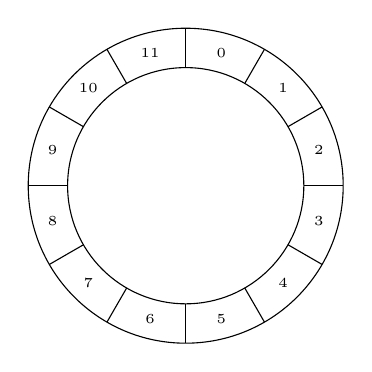
\begin{tikzpicture}[scale=.5]
				\def\RayonListe{3}
				\def\EpaisseurListe{1}
				\def\LongueurListe{12}
				\draw (0,0) circle(\RayonListe);
				\draw (0,0) circle(\RayonListe+\EpaisseurListe);
				\foreach \compt in {0,1,...,\numexpr\LongueurListe-1}
				{
					\draw (90-\compt/\LongueurListe*360:\RayonListe)--(90-\compt/\LongueurListe*360:\RayonListe+\EpaisseurListe);
					\draw (90-\compt/\LongueurListe*360-180/\LongueurListe:\RayonListe+\EpaisseurListe/2)node{\tiny \compt};
				}
				\end{tikzpicture}
		\end{center}}{6cm}
		
		\item 	\ \\\double{
			Refaire \textbf{1.} et \textbf{2.} mais en sautant 5 cases.\\
			Case parcourues : \dotfill\\}
		{
			\begin{center}
				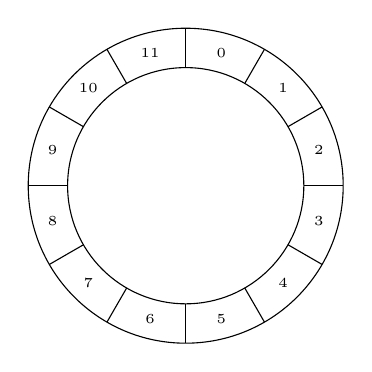
\begin{tikzpicture}[scale=.5]
				\def\RayonListe{3}
				\def\EpaisseurListe{1}
				\def\LongueurListe{12}
				\draw (0,0) circle(\RayonListe);
				\draw (0,0) circle(\RayonListe+\EpaisseurListe);
				\foreach \compt in {0,1,...,\numexpr\LongueurListe-1}
				{
					\draw (90-\compt/\LongueurListe*360:\RayonListe)--(90-\compt/\LongueurListe*360:\RayonListe+\EpaisseurListe);
					\draw (90-\compt/\LongueurListe*360-180/\LongueurListe:\RayonListe+\EpaisseurListe/2)node{\tiny \compt};
				}
				\end{tikzpicture}
		\end{center}}{6cm}
		\item 	Comment expliquer la différence entre la dernière liste et les deux premières ?\\
	\end{enumerate}
\end{exercice}


\begin{exercice}[]
	On parcourt une liste circulaire de longueur 84 comme à l'exercice précédent, en partant de la case d'indice zéro et en sautant 735 cases (et oui 
	cela fait beaucoup) à chaque fois, indéfiniment.\\
	La liste sera-t-elle parcourue entièrement ? Si ce n'est pas le cas, donner la liste des cases parcourues.\\
	\textit{Justifier les réponses}.
	
	
\end{exercice}

\end{document}
